\documentclass[12pt,a4paper]{article}
\usepackage[utf8]{inputenc}
\usepackage[russian]{babel}
\usepackage{amsmath,amssymb,amsthm}
\usepackage{geometry}
\geometry{left=2cm,right=2cm,top=2cm,bottom=2cm}
\usepackage{enumitem}
\usepackage{tikz}
\usetikzlibrary{automata,positioning}

\theoremstyle{definition}
\newtheorem{definition}{Определение}[section]
\newtheorem{theorem}{Теорема}[section]
\newtheorem{lemma}{Лемма}[section]
%\newtheorem{proof}{Доказательство}[section]
\newtheorem{example}{Пример}[section]

\newcommand{\lang}{\mathcal{L}}
\newcommand{\set}[1]{\{#1\}}
\newcommand{\emptystring}{\varepsilon}
\newcommand{\N}{\mathbb{N}}
\newcommand{\A}{\mathcal{A}}
\newcommand{\RE}{\text{RE}}

\title{Основные понятия формальных языков и грамматик\\
Классификация Хомского, автоматы и леммы о разрастании\\
\large{Расширенный конспект с доказательствами}}
\author{}
\date{}

\begin{document}

\maketitle

\section{Введение: алфавиты, слова, языки}

\begin{definition}
\textbf{Алфавит} --- конечное непустое множество символов. Обозначается $\Sigma$.
\end{definition}

\begin{definition}
\textbf{Слово (цепочка)} над $\Sigma$ --- конечная последовательность символов из $\Sigma$. Длина $|w|$ --- число символов. Пустое слово $\emptystring$.
\end{definition}

\begin{definition}
\textbf{Язык} $L$ над $\Sigma$ --- произвольное множество слов над $\Sigma$.
\end{definition}

Операции: объединение $L_1\cup L_2$, пересечение $L_1\cap L_2$, конкатенация $L_1L_2 = \{uv\mid u\in L_1, v\in L_2\}$, итерация (звезда Клини) $L^* = \bigcup_{i\ge 0} L^i$, где $L^0=\{\emptystring\}$.

\section{Формальные грамматики}

\begin{definition}
\textbf{Порождающая грамматика} $G = (N, \Sigma, P, S)$, где $N$ --- нетерминалы, $\Sigma$ --- терминалы, $P$ --- конечное множество правил $\alpha\to\beta$, $\alpha$ содержит хотя бы один нетерминал, $S\in N$ --- начальный символ.
\end{definition}

Отношение непосредственного вывода: $\gamma\alpha\delta \Rightarrow \gamma\beta\delta$, если $\alpha\to\beta\in P$. Рефлексивно-транзитивное замыкание $\Rightarrow^*$. \textbf{Язык грамматики}: $L(G) = \{w\in\Sigma^* \mid S\Rightarrow^* w\}$.

\begin{example}
Рассмотрим грамматику $G = (N, \Sigma, P, S)$, порождающую язык $\{a^n b^n c^n \mid n \ge 1\}$:
\begin{itemize}
\item $N = \{S, A, B, C, D, E\}$ --- нетерминалы (вспомогательные символы);
\item $\Sigma = \{a, b, c\}$ --- терминалы (символы итоговых слов);
\item $P$ содержит правила:
  \[
  \begin{array}{ll}
  S \to aSBC \mid aBC, & \text{(порождаем равное количество $a$, $B$, $C$)} \\
  CB \to BC,            & \text{(перестановка для порядка $b$ и $c$)} \\
  aB \to ab,            & \text{(превращаем $B$ в $b$ после $a$)} \\
  bB \to bb,            & \text{(продолжаем замену $B$ на $b$)} \\
  bC \to bc,            & \text{(начинаем замену $C$ на $c$)} \\
  cC \to cc.            & \text{(завершаем замену $C$)}
  \end{array}
  \]
\end{itemize}

\textbf{Пример вывода для $n=2$ ($a^2 b^2 c^2$):}
\[
\begin{aligned}
S &\Rightarrow aSBC \Rightarrow a(aBC)BC = aaBCBC \\
  &\Rightarrow aaB CBC \Rightarrow aaB BCC \Rightarrow aabBCC \\
  &\Rightarrow aabbCC \Rightarrow aabbcC \Rightarrow aabbcc.
\end{aligned}
\]
\end{example}

\section{Классификация грамматик по Хомскому}

\begin{definition}[Тип 0]
Грамматики без ограничений. Соответствуют рекурсивно перечислимым языкам.
\end{definition}

\begin{definition}[Тип 1, контекстно-зависимые]
Правила $\alpha A\beta \to \alpha\gamma\beta$, где $A\in N$, $\gamma\neq\emptystring$ (разрешён $S\to\emptystring$ при условии, что $S$ не встречается в правых частях).
\end{definition}

\begin{definition}[Тип 2, контекстно-свободные (КС)]
Правила $A\to\gamma$, $A\in N$, $\gamma\in (N\cup\Sigma)^*$.
\end{definition}

\begin{definition}[Тип 3, регулярные]
Правила $A\to aB$, $A\to a$ или $A\to\emptystring$, $A,B\in N$, $a\in\Sigma$.
\end{definition}

\subsection*{Включения классов}
\begin{theorem}
Тип 3 $\subset$ тип 2 $\subset$ тип 1 $\subset$ тип 0. Все включения строгие.
\end{theorem}

\begin{proof}[Доказательство строгости включений]
\begin{itemize}
\item \textbf{Тип 3 $\subset$ тип 2:} Любая регулярная грамматика является КС-грамматикой (правила вида $A\to aB$ и $A\to a$ уже удовлетворяют определению КС). Обратное неверно: язык $\{a^n b^n \mid n\ge 0\}$ порождается КС-грамматикой $S\to aSb\mid\emptystring$, но не является регулярным (доказывается леммой о разрастании для регулярных языков, см. раздел \ref{sec:pumping-reg}).
\item \textbf{Тип 2 $\subset$ тип 1:} КС-грамматика может иметь правила $A\to\emptystring$, что недопустимо в контекстно-зависимых (кроме $S\to\emptystring$). Однако любую КС-грамматику можно преобразовать в эквивалентную контекстно-зависимую (удалив $\emptystring$-правила и заменив их правилами вида $\alpha A\beta \to \alpha\gamma\beta$). Язык $\{a^n b^n c^n \mid n\ge 0\}$ является контекстно-зависимым (грамматика: $S\to aSBC\mid aBC$, $CB\to BC$, $aB\to ab$, $bB\to bb$, $bC\to bc$, $cC\to cc$), но не КС (доказывается леммой о разрастании для КС-языков, раздел \ref{sec:pumping-cfl}).
\item \textbf{Тип 1 $\subset$ тип 0:} Любая контекстно-зависимая грамматика является грамматикой типа 0. Существуют рекурсивно перечислимые языки, не являющиеся контекстно-зависимыми. Пример: язык, распознаваемый универсальной машиной Тьюринга (проблема остановки). Контекстно-зависимые языки всегда разрешимы (алгоритм работает, перебирая выводы ограниченной длины), а рекурсивно перечислимые могут быть неразрешимы.
\end{itemize}
\end{proof}

\section{Регулярные языки и конечные автоматы}

\begin{definition}
ДКА --- пятерка $\A = (Q, \Sigma, \delta, q_0, F)$, где $Q$ --- конечное множество состояний, $\delta: Q\times\Sigma\to Q$ --- функция переходов, $q_0$ --- начальное состояние, $F\subseteq Q$ --- множество допускающих состояний. Распознавание: $\hat\delta(q_0,w)\in F$.
\end{definition}

\subsection{Недетерминированные конечные автоматы (НКА)}

\begin{definition}
НКА отличается от ДКА тем, что $\delta: Q\times(\Sigma\cup\{\emptystring\})\to 2^Q$ (множество возможных состояний). Слово допускается, если существует путь из $q_0$ в какое-либо $f\in F$ по меткам слова с возможными $\emptystring$-переходами.
\end{definition}

\subsection{Регулярные выражения}
Определяются рекурсивно: $\varnothing$, $\emptystring$, $a\in\Sigma$, и если $r,s$ --- выражения, то $(r|s)$, $(rs)$, $(r^*)$. Язык, задаваемый выражением, обозначается $L(r)$.

\subsection{Теорема Клини (доказательство)}
\begin{theorem}[Клини]
Класс языков, задаваемых регулярными выражениями, совпадает с классом языков, распознаваемых конечными автоматами (ДКА или НКА).
\end{theorem}

\begin{proof}
Докажем в двух направлениях.

\textbf{1. По регулярному выражению строим НКА.}
Индукция по построению выражения:
\begin{itemize}
\item $\varnothing$: автомат без допускающих состояний.
\item $\emptystring$: автомат с $q_0\in F$.
\item $a$: автомат $q_0\xrightarrow{a} q_1$, $q_1$ допускающий.
\item $r|s$: строим НКА с новым начальным состоянием, $\emptystring$-переходами в начальные состояния автоматов для $r$ и $s$, и объединяем допускающие состояния (с $\emptystring$-переходами в общее новое допускающее).
\item $rs$: последовательное соединение: $\emptystring$-переход из допускающих состояний первого автомата в начальное состояние второго.
\item $r^*$: добавляем новое начальное и допускающее состояние, $\emptystring$-переходы: из нового начала в старое начало и в новое допускающее; из старых допускающих в старое начало и новое допускающее.
\end{itemize}
Полученный НКА имеет не более чем в $2n+1$ раз больше состояний, где $n$ --- размер выражения.

\textbf{2. По ДКА строим регулярное выражение.}
Пусть ДКА $\A = (\{1,\dots,n\},\Sigma,\delta,1,F)$. Определим $R_{ij}^{(k)}$ --- множество слов, которые переводят автомат из состояния $i$ в состояние $j$, используя только промежуточные состояния с номерами $\le k$. Рекурсия:
\[
R_{ij}^{(0)} = 
\begin{cases}
\{a\mid \delta(i,a)=j\} \cup \{\emptystring\} & \text{если } i=j,\\
\{a\mid \delta(i,a)=j\} & \text{иначе}.
\end{cases}
\]
\[
R_{ij}^{(k)} = R_{ij}^{(k-1)} | R_{ik}^{(k-1)} (R_{kk}^{(k-1)})^* R_{kj}^{(k-1)}.
\]
Язык автомата $L(\A) = \bigcup_{j\in F} R_{1j}^{(n)}$. Каждое $R_{ij}^{(k)}$ представляется регулярным выражением (индукция по $k$). Таким образом, получаем регулярное выражение для $L(\A)$. Для НКА сначала преобразуем в ДКА методом подмножеств (см. раздел \ref{sec:nfa2dfa}).
\end{proof}

\subsection{Классы Майхилла–Нероды и минимизация ДКА}

\begin{definition}
Отношение правой инвариантности: $x\equiv_L y$, если $\forall z\in\Sigma^*: xz\in L \iff yz\in L$. Индекс $L$ --- число классов эквивалентности.
\end{definition}

\begin{theorem}[Майхилл–Нерода]
$L$ регулярен $\iff$ $\equiv_L$ имеет конечный индекс. Минимальный ДКА для $L$ имеет число состояний, равное индексу $L$.
\end{theorem}

\begin{proof}
($\Rightarrow$) Если $L$ регулярен, существует ДКА $\A$ с $m$ состояниями. Определим отображение $\varphi(w)=\hat\delta(q_0,w)$. Если $\varphi(x)=\varphi(y)$, то $x\equiv_L y$. Следовательно, классов не больше $m$. ($\Leftarrow$) Если индекс конечен, построим ДКА: состояния = классы эквивалентности $[w]$, начальное $[\emptystring]$, переход $[w]\xrightarrow{a}[wa]$, допускающие --- классы, содержащие слова из $L$. Этот автомат распознаёт $L$ и минимален (любой автомат с меньшим числом состояний бы не смог отличить какие-то из классов эквивалентности $\equiv_L$).
\end{proof}

\subsection{Минимизация ДКА (алгоритм Хопкрофта)}
Минимизация ДКА позволяет по любому ДКА построить эквивалентный ему ДКА с наименьшим возможным числом состояний. Минимальный автомат единствен с точностью до изоморфизма.

\subsubsection{Основная идея}

Два состояния $p$ и $q$ называются \textbf{неразличимыми} (эквивалентными), если для любого слова $w\in\Sigma^*$ автомат, начав из $p$ и из $q$, после прочтения $w$ либо оба оказываются в допускающих состояниях, либо оба в недопускающих. В противном случае состояния различимы.

Минимальный автомат получается склеиванием всех неразличимых состояний в один класс.

\subsubsection{Алгоритм Хопкрофта (табличный метод)}

Пусть дан ДКА $\A = (Q, \Sigma, \delta, q_0, F)$. Алгоритм строит разбиение множества $Q$ на классы неразличимых состояний.

\begin{enumerate}
\item \textbf{Начальное разбиение:} $\Pi_0 = \{F,\; Q\setminus F\}$ (допускающие и недопускающие состояния заведомо различимы, так как пустое слово их различает).

\item \textbf{Итеративное уточнение:} На каждом шаге для текущего разбиения $\Pi$ проверяем каждую группу $G\in\Pi$ и каждый символ $a\in\Sigma$: если переходы по $a$ из состояний $G$ ведут в разные группы текущего разбиения, то $G$ расщепляется на подгруппы состояний, у которых образы по $a$ лежат в одной и той же группе.

Формально: для $G\in\Pi$ и $a\in\Sigma$ определим отображение $\delta_a(G) = \{\delta(q,a) \mid q\in G\}$. Разобьём $G$ на классы эквивалентности по отношению $q_1 \sim_a q_2$, если $\delta(q_1,a)$ и $\delta(q_2,a)$ принадлежат одному блоку $\Pi$. Полученные подгруппы заменяют $G$ в новом разбиении.

\item \textbf{Критерий остановки:} Если на очередной итерации разбиение не изменилось ($\Pi_{k+1} = \Pi_k$), алгоритм завершается.

\item \textbf{Построение минимального автомата:} Каждый блок результирующего разбиения становится одним состоянием. Начальный блок — тот, который содержит $q_0$. Допускающие блоки — те, которые содержат состояния из $F$. Переход из блока $B$ по символу $a$ ведёт в блок, содержащий $\delta(q,a)$ для любого $q\in B$ (определение корректно, так как состояния в блоке неразличимы).
\end{enumerate}

\subsubsection{Доказательство корректности}

\begin{proof}
\textbf{Лемма 1:} Если два состояния различимы, то алгоритм рано или поздно поместит их в разные блоки.  
Действительно, различие означает существование слова $w = a_1\dots a_k$, которое переводит одно состояние в допускающее, а другое — в нет. При разборе по символам с конца можно показать, что на некотором шаге они попадут в разные группы при расщеплении по последнему символу.

\textbf{Лемма 2:} Если алгоритм поместил состояния в один блок, то они неразличимы.  
Индукция по длине слова: база (пустое слово) — они оба либо допускающие, либо нет (иначе были бы в разных блоках с самого начала). Шаг: пусть для всех слов длины $<n$ они ведут себя одинаково. Рассмотрим слово $w=av$. По построению, $\delta(p,a)$ и $\delta(q,a)$ лежат в одном блоке (иначе $p$ и $q$ расщепились бы на шаге по $a$). По индуктивному предположению, эти состояния неразличимы на $v$, значит, $p$ и $q$ неразличимы на $av$.

Таким образом, финальное разбиение в точности соответствует отношению неразличимости, а число блоков минимально.
\end{proof}

\subsection{Пример минимизации}

Рассмотрим ДКА, распознающий язык $$L = \{w \in \{0,1\}^* \mid w \text{ содержит чётное число нулей и чётное число единиц}\}.$$ Состояния: $(\operatorname{parity}_0, \operatorname{parity}_1)$. Всего 4 состояния. Начальное $(0,0)$ допускающее.

Алгоритм:
\begin{itemize}
\item Начальное разбиение: $\Pi_0 = \{\{(0,0)\},\; \{(0,1),(1,0),(1,1)\}\}$ (допускающее одно).
\item По символу $0$: $(0,0)\to(1,0)$ (недопускающее), $(0,1)\to(1,1)$ (недопускающее), $(1,0)\to(0,0)$ (допускающее), $(1,1)\to(0,1)$ (недопускающее). Среди недопускающих $(0,1)$ и $(1,1)$ идут в разные блоки? Нет: $(0,1)\to(1,1)$ (в блоке недопускающих), $(1,1)\to(0,1)$ (тоже в недопускающих). Но $(1,0)\to(0,0)$ (допускающий блок). Значит, недопускающие разбиваются на две группы: те, кто по $0$ идёт в допускающий ($(1,0)$), и те, кто идёт в недопускающий ($(0,1)$ и $(1,1)$). Аналогично по $1$ уточняем. В итоге получим 4 отдельных состояния — автомат уже минимален.
\end{itemize}

\section{Преобразование НКА в ДКА (метод подмножеств)}\label{sec:nfa2dfa}
Недетерминизм даёт краткость описания, но для практической реализации (например, в лексических анализаторах) удобнее детерминированный автомат. Метод подмножеств (subset construction) позволяет по любому НКА построить эквивалентный ДКА.

\subsection{Словесное описание алгоритма}

Пусть дан НКА $\A = (Q, \Sigma, \delta, q_0, F)$. Идея: каждое состояние ДКА будет представлять \textbf{множество состояний} исходного НКА, в которых автомат может оказаться после прочтения некоторого слова. Так как $Q$ конечно, множество всех подмножеств $2^Q$ конечно, поэтому ДКА будет иметь не более $2^{|Q|}$ состояний (на практике достижимых гораздо меньше).

\textbf{Шаг 1: $\varepsilon$-замыкание.} Для любого множества $R\subseteq Q$ определим $\varepsilon\text{-closure}(R)$ как множество состояний, достижимых из $R$ с помощью нуля или более $\varepsilon$-переходов (не читая входных символов). Это легко вычислить обходом графа $\varepsilon$-переходов.

\textbf{Шаг 2: Построение переходов ДКА.}  
Состояниями ДКА будут подмножества $Q$ (и только те, которые достижимы из начального). Начальное состояние ДКА — $S_0 = \varepsilon\text{-closure}(\{q_0\})$.  
Для каждого состояния-подмножества $T$ (уже построенного) и каждого символа $a\in\Sigma$:
\begin{enumerate}
\item Находим все состояния, в которые можно перейти из любого $q\in T$ по символу $a$: $U = \bigcup_{q\in T} \delta(q,a)$.
\item Затем берём $\varepsilon$-замыкание $U$: $T' = \varepsilon\text{-closure}(U)$.
\item Это $T'$ становится состоянием ДКА, и добавляем переход $T \xrightarrow{a} T'$.
\end{enumerate}
Если $T'$ ещё не встречалось, добавляем его в множество состояний ДКА для дальнейшей обработки.

\textbf{Шаг 3: Допускающие состояния ДКА.} Состояние-подмножество $T$ является допускающим в ДКА, если $T$ содержит хотя бы одно допускающее состояние исходного НКА (т.е. $T\cap F \neq \varnothing$). Это соответствует тому, что существует путь, заканчивающийся в допускающем состоянии.

\textbf{Шаг 4: Удаление недостижимых состояний.} После построения всех достижимых подмножеств (алгоритм BFS/DFS по графу ДКА) остаются только те состояния, которые действительно нужны.

\subsection{Обоснование корректности}

\begin{proof}
Докажем по индукции по длине слова $w$, что после прочтения $w$ в ДКА мы оказываемся в состоянии $\hat\delta_{DFA}(S_0, w)$, которое в точности равно множеству всех состояний НКА, достижимых из $q_0$ по слову $w$ (с учётом $\varepsilon$-переходов).  
База: $|w|=0$, $w=\emptystring$. Тогда $\hat\delta_{DFA}(S_0,\emptystring)=S_0 = \varepsilon\text{-closure}(\{q_0\})$ — по определению это все состояния, достижимые без чтения символов.  
Индукционный переход: пусть для $w$ утверждение верно. Рассмотрим $wa$. По построению ДКА, $\delta_{DFA}( \hat\delta_{DFA}(S_0,w), a) = \varepsilon\text{-closure}\left(\bigcup_{q\in \hat\delta_{DFA}(S_0,w)} \delta(q,a)\right)$. Внутри объединения — все состояния, достижимые из $q_0$ по $w$ (по индукции), затем по $a$, затем $\varepsilon$-замыкание. Это в точности множество состояний НКА, достижимых по $wa$.  
Слово $wa$ допускается ДКА тогда и только тогда, когда это множество содержит допускающее состояние НКА, что эквивалентно существованию пути в НКА, оканчивающегося в допускающем состоянии. Таким образом, языки совпадают.
\end{proof}

\subsection{Пример преобразования}

Рассмотрим НКА для $L = \{0^n \mid n\ge 0\} \cup \{1^n \mid n\ge 0\}$:
\begin{center}
\begin{tikzpicture}[shorten >=1pt,node distance=2cm,on grid,auto]
\node[state,initial] (q0) {$q_0$};
\node[state,accepting] (q1) [right=of q0] {$q_1$};
\node[state,accepting] (q2) [below=of q0] {$q_2$};
\draw[->] (q0) edge node {$\varepsilon$} (q1);
\draw[->] (q0) edge node {$\varepsilon$} (q2);
\draw[->] (q1) edge [loop above] node {$0$} (q1);
\draw[->] (q2) edge [loop below] node {$1$} (q2);
\end{tikzpicture}
\end{center}
$Q=\{q_0,q_1,q_2\}$, $F=\{q_1,q_2\}$.

\paragraph{Метод подмножеств:}
\begin{itemize}
\item $\varepsilon\text{-closure}(\{q_0\}) = \{q_0,q_1,q_2\} =: A$ (начальное состояние ДКА).
\item Из $A$ по $0$: $\delta(q_1,0)=\{q_1\}$ → $\{q_1\}=:B$.
\item Из $A$ по $1$: $\delta(q_2,1)=\{q_2\}$ → $\{q_2\}=:C$.
\item Из $B$ по $0$: $\{q_1\}$ → $B$; по $1$: $\varnothing=:D$.
\item Из $C$ по $0$: $\varnothing$ → $D$; по $1$: $\{q_2\}$ → $C$.
\item Из $D$ по $0,1$: $\varnothing$ → $D$.
\end{itemize}
Допускающие: $A,B,C$ (содержат $q_1$ или $q_2$). Полученный ДКА имеет 4 состояния, эквивалентен исходному НКА.

\begin{center}
\begin{tikzpicture}[shorten >=1pt,node distance=2.5cm,on grid,auto]
\node[state,initial,accepting] (A) {$A$};
\node[state,accepting] (B) [right=of A] {$B$};
\node[state,accepting] (C) [below=of A] {$C$};
\node[state] (D) [below=of B] {$D$};

\draw[->] (A) edge node {$0$} (B);
\draw[->] (A) edge node {$1$} (C);
\draw[->] (B) edge [loop above] node {$0$} (B);
\draw[->] (B) edge node {$1$} (D);
\draw[->] (C) edge node {$0$} (D);
\draw[->] (C) edge [loop below] node {$1$} (C);
\draw[->] (D) edge [loop right] node {$0,1$} (D);
\end{tikzpicture}
\end{center}

\subsection{Замечания}
\begin{itemize}
\item Метод подмножеств применим к любому НКА, в том числе с $\varepsilon$-переходами (предварительно вычисляется $\varepsilon$-замыкание).
\item В худшем случае число состояний ДКА экспоненциально относительно числа состояний НКА, но на практике часто получается разумное количество.
\item Полученный ДКА, вообще говоря, не обязательно минимален; его можно дополнительно минимизировать алгоритмом из предыдущего раздела.
\end{itemize}

\section{Лемма о разрастании для регулярных языков}\label{sec:pumping-reg}
\begin{lemma}[Pumping lemma]
Для любого регулярного языка $L$ существует $p\ge 1$ (длина накачки), такое что для любого $w\in L$ с $|w|\ge p$ найдутся $x,y,z$: $w=xyz$, $|xy|\le p$, $|y|\ge 1$ и $\forall i\ge0: xy^iz\in L$.
\end{lemma}

\begin{proof}
Пусть $L$ распознаётся ДКА с $n$ состояниями. Возьмём $p=n$. Для $w$ длины $\ge n$ при чтении первых $n$ символов (прошли $n+1$ состояние, включая начальное) встретим повторяющееся состояние. Пусть $q$ --- первое повторяющееся состояние, $x$ --- часть до первого вхождения $q$, $y$ --- между первым и вторым вхождением, $z$ --- остаток. Тогда $|xy|\le n$, $|y|\ge1$. Для любого $i$ путь по $xy^iz$ также допустим (повторяем цикл $y$ $i$ раз).
\end{proof}

Применение: язык $\{a^n b^n \mid n\ge0\}$ не регулярен. Допустим, он регулярен с $p$. Возьмём $w=a^p b^p$. По лемме $y$ состоит только из $a$ (так как $|xy|\le p$). Тогда $xy^2z$ содержит больше $a$, чем $b$, противоречие.

\section{Контекстно-свободные грамматики}

\subsection{Деревья вывода}
Дерево вывода: корень $S$, внутренние узлы --- нетерминалы, дети соответствуют правой части правила. Листья --- терминалы или $\emptystring$. Левое (правое) порождение всегда раскрывает самый левый (правый) нетерминал.

Грамматика \textbf{неоднозначна}, если существует слово с двумя различными деревьями вывода. Пример: $S\to S+S\mid a$ неоднозначна, так как $a+a+a$ имеет два дерева.

\subsection{Нормальные формы}

\begin{definition}[Нормальная форма Хомского (CNF)]
Все правила $A\to BC$ или $A\to a$, где $A,B,C\in N$, $a\in\Sigma$. Допускается $S\to\emptystring$.
\end{definition}

\begin{definition}[Нормальная форма Грейбах (GNF)]
Правила $A\to a\gamma$, $a\in\Sigma$, $\gamma\in N^*$.
\end{definition}

\subsubsection{Алгоритм приведения КС-грамматики к нормальной форме Хомского (CNF)}

\paragraph{Шаг 1: Замена терминалов в правых частях правил.}
Для каждого терминала $c \in \Sigma$, встречающегося в правой части правила, вводим новый нетерминал $G_c$ и добавляем правило $G_c \to c$. Затем в каждом исходном правиле $A \to \alpha$ заменяем каждое вхождение терминала $c$ на $G_c$.

\paragraph{Шаг 2: Бинаризация (разбиение длинных правил).}
Для каждого правила вида $A \to X_1 X_2 \ldots X_k$ с $k \ge 3$ (где $X_i$ --- нетерминалы, возможно, $G_c$) вводим новые нетерминалы $D_1, D_2, \ldots, D_{k-2}$ и заменяем правило на набор:
\[
A \to X_1 D_1,\quad D_1 \to X_2 D_2,\quad \ldots,\quad D_{k-2} \to X_{k-1} X_k.
\]
Теперь все правила имеют один из четырёх типов:
\begin{itemize}
\item $A \to \varepsilon$ (если исходная грамматика содержала $\varepsilon$-правила),
\item $G_c \to c$ (терминальные правила),
\item $A \to B$ (цепные правила, где $B$ --- нетерминал),
\item $A \to BC$ (правила с двумя нетерминалами).
\end{itemize}

\paragraph{Шаг 3: Устранение $\varepsilon$-правил.}
\begin{enumerate}
\item Найти множество $E$ \textbf{аннулирующих} ($\varepsilon$-порождающих) нетерминалов: $A \in E$ если $A \Rightarrow^* \varepsilon$.
   Итеративно: если есть правило $A \to \varepsilon$, то $A \in E$; если есть правило $A \to X_1\ldots X_m$ и все $X_i \in E$, то $A \in E$.
\item Для каждого правила вида $A \to BC$ ($B,C$ --- нетерминалы) добавить новые правила:
   \begin{itemize}
   \item Если $B \in E$, то из $A \to BC$ добавляем $A \to C$.
   \item Если $C \in E$, то из $A \to BC$ добавляем $A \to B$.
   \end{itemize}
\item Удалить все правила вида $A \to \varepsilon$. Если $S \in E$, то добавить $S \to \varepsilon$ в грамматику.
\end{enumerate}

\paragraph{Шаг 4: Устранение цепных правил (правил вида $A \to B$, где $B \in N$).}
\begin{enumerate}
\item Построить граф цепных зависимостей: вершины --- нетерминалы, ребро $A \to B$ если есть цепное правило.
\item Для каждого нетерминала $A$ вычислить замыкание $\operatorname{Chain}(A)$ --- множество всех нетерминалов, достижимых из $A$ по цепным правилам (включая $A$).
\item Для каждого $B \in \operatorname{Chain}(A)$ и каждого \textbf{нецепного} правила $B \to \gamma$ (где $\gamma$ не является одним нетерминалом, т.е. $\gamma = c$ или $\gamma = CD$), добавить правило $A \to \gamma$.
\item Удалить все цепные правила.
\end{enumerate}

\paragraph{Шаг 5: (Опционально) Удаление бесполезных символов.}
Выполнить стандартные процедуры удаления непорождающих и недостижимых символов (после всех преобразований).

\paragraph{Пример:}
Исходная грамматика $S \to aSb \mid \varepsilon$.
\begin{itemize}
\item Шаг 1: Вводим $G_a \to a$, $G_b \to b$. Правило $S \to G_a S G_b$.
\item Шаг 2: Бинаризация: $S \to G_a D$, $D \to S G_b$.
\item Шаг 3: Находим аннулирующие: $S$ аннулирующий (из $S\to\varepsilon$).
   Добавляем правила из $D \to S G_b$: $S\in E$ → добавляем $D \to G_b$.
   Оставляем $S\to\varepsilon$ как исключение для начального нетерминала.
   Теперь имеем: $S \to G_a D \mid \varepsilon$, $D \to S G_b \mid G_b$, $G_a\to a$, $G_b\to b$.
\item Шаг 4: Цепные правила: $D \to G_b$ (цепное, $G_b$ нетерминал). $\operatorname{Chain}(D)=\{D, G_b\}$. Для $G_b$ есть нецепное $G_b\to b$, добавляем $D\to b$. Удаляем $D\to G_b$. Цепных больше нет.
\item Итоговая CNF: $S \to G_a D \mid \varepsilon$, $D \to S G_b \mid b$, $G_a \to a$, $G_b \to b$.
\end{itemize}
\subsection{Лемма о разрастании для КС-языков}\label{sec:pumping-cfl}
\begin{lemma}[Pumping lemma для КС-языков]
Для любого КС-языка $L$ существует $p>0$, такое что любое $w\in L$ с $|w|\ge p$ представимо как $w=uvxyz$, где $|vxy|\le p$, $|vy|\ge1$, и $\forall i\ge0: uv^ixy^iz\in L$.
\end{lemma}

\begin{proof}
Рассмотрим грамматику $G$ в CNF для $L$ (без $\emptystring$-правил). Пусть $m$ --- число нетерминалов. Выберем $p=2^m$. Для слова $w$ длины $\ge p$ дерево вывода имеет высоту $\ge m+1$ (так как в CNF каждое правило увеличивает длину строки не более чем вдвое). На пути от корня к листу длиной $>m$ встретится повторяющийся нетерминал $A$. Пусть $vxy$ --- подстрока, выводимая из второго вхождения $A$, и $A\Rightarrow^* vAy$ и $A\Rightarrow^* x$. Тогда можно заменить $A$ на $vAy$ любое число раз (накачка). Ограничение $|vxy|\le p$ следует из выбора $p$ (можно выбрать первое повторение на достаточно малой высоте).
\end{proof}

Применение: язык $\{a^n b^n c^n\}$ не КС. Предположим, он КС с $p$. Возьмём $a^p b^p c^p$. По лемме $vxy$ не может содержать все три символа (иначе $|vxy|$ слишком мал, чтобы покрыть расстояния). Возможны два случая: $vxy$ не содержит $a$ или не содержит $c$. При накачке нарушится равенство чисел $a$, $b$, $c$.

\section{Детерминированные и недетерминированные КС-грамматики}

КС-грамматика называется однозначной, если у каждого слова имеется не более одного дерева разбора в этой грамматике. Множество языков, задающихся однозначными КС-грамматиками, называется DCFL. Множество языков, задающихся неоднозначными КС-грамматиками, называется NCFL. Один и тот же КС-язык может задаваться одновременно и однозначной, и неоднозначной грамматикой. Обратно, существуют КС-языки, которые могут задаваться только неоднозначной грамматикой. Пример NCFL, не являющегося DCFL: $\{a^n b^m \mid n=m \text{ или } n=2m\}$.

\section{Автоматы с магазинной памятью (МП-автоматы)}

Автомат с магазинной памятью (pushdown automaton, PDA) — это расширение конечного автомата, снабжённое стеком. Стек позволяет запоминать неограниченное количество информации (но доступ к ней осуществляется только сверху). Именно это даёт возможность распознавать контекстно-свободные языки.

\begin{definition}
\textbf{МП-автомат} (недетерминированный) задаётся семёркой:
\[
M = (Q, \Sigma, \Gamma, \delta, q_0, Z_0, F),
\]
где:
\begin{itemize}
\item $Q$ — конечное множество \textbf{состояний};
\item $\Sigma$ — \textbf{входной алфавит} (терминалы);
\item $\Gamma$ — \textbf{стековый алфавит} (символы, которые можно класть в стек);
\item $\delta$ — \textbf{функция переходов}: 
\[
\delta: Q \times (\Sigma \cup \{\varepsilon\}) \times \Gamma \longrightarrow 2^{Q \times \Gamma^*};
\]
\item $q_0 \in Q$ — \textbf{начальное состояние};
\item $Z_0 \in \Gamma$ — \textbf{начальный символ стека} (дно стека);
\item $F \subseteq Q$ — множество \textbf{допускающих состояний}.
\end{itemize}
\end{definition}

\paragraph{Пояснение к функции переходов.}
Аргументы: текущее состояние, следующий входной символ (или $\varepsilon$, означающий, что вход не читается), и верхний символ стека (который извлекается при выполнении перехода). Результат: конечное множество пар $(q', \gamma)$, где $q'$ — новое состояние, а $\gamma$ — строка символов, которая \textbf{заменяет} верхушку стека (т.е. удалённый символ заменяется на $\gamma$; если $\gamma = \varepsilon$, то стек просто уменьшается на один элемент; если $\gamma = XY$, то сначала удаляется верхний символ, затем на его место кладутся $X, Y$ в указанном порядке, причём $X$ становится новым верхним).

\paragraph{Конфигурация и такт работы.}
\textbf{Конфигурация} — тройка $(q, w, \alpha) \in Q \times \Sigma^* \times \Gamma^*$, где $q$ — состояние, $w$ — остаток входной цепочки (её начало уже прочитано), $\alpha$ — содержимое стека (первый символ — вершина).  
\textbf{Такт перехода} (обозначается $\vdash$): $(q, aw, \beta X) \vdash (q', w, \beta\gamma)$, если $(q', \gamma) \in \delta(q, a, X)$, где $a \in \Sigma \cup \{\varepsilon\}$, $X \in \Gamma$. Если $a = \varepsilon$, то вход не читается ($aw = w$).  
Рефлексивно-транзитивное замыкание $\vdash^*$ обозначает произвольное число тактов.

\paragraph{Допускание.}
МП-автомат $M$ допускает слово $w$, если
\[
(q_0, w, Z_0) \vdash^* (q, \varepsilon, \alpha)
\]
для некоторого $q \in F$ (допускающее состояние) и произвольного $\alpha \in \Gamma^*$ (стек может быть любым).  
Существует также эквивалентное определение допускания по \textbf{пустому стеку} (независимо от состояния) — оба варианта эквивалентны по выразительной силе.

\paragraph{Пример МП-автомата для языка $\{a^n b^n \mid n \ge 0\}$.}
\begin{itemize}
\item $Q = \{q_0, q_1, q_2\}$, $\Sigma = \{a,b\}$, $\Gamma = \{A, Z_0\}$, начальное состояние $q_0$, начальный стек $Z_0$, допускающее состояние $q_2$.
\item Переходы:
  \begin{itemize}
  \item $\delta(q_0, a, Z_0) = \{(q_0, A Z_0)\}$ — кладём $A$ в стек (счётчик нулей).
  \item $\delta(q_0, a, A) = \{(q_0, A A)\}$ — увеличиваем счётчик.
  \item $\delta(q_0, b, A) = \{(q_1, \varepsilon)\}$ — встречаем $b$, начинаем извлекать $A$.
  \item $\delta(q_1, b, A) = \{(q_1, \varepsilon)\}$ — продолжаем извлекать.
  \item $\delta(q_1, \varepsilon, Z_0) = \{(q_2, Z_0)\}$ — стек опустел, переходим в допускающее состояние.
  \end{itemize}
\end{itemize}
Работа на слове $a^2 b^2$:
\[
(q_0, aabb, Z_0) \vdash (q_0, abb, A Z_0) \vdash (q_0, bb, A A Z_0) \vdash (q_1, b, A Z_0) \vdash (q_1, \varepsilon, Z_0) \vdash (q_2, \varepsilon, Z_0).
\]

\begin{theorem}
Класс языков, допускаемых МП-автоматами (недетерминированными), совпадает с классом КС-языков.
\end{theorem}

\begin{proof}[Конструкция]
($\Rightarrow$) По МП-автомату строим КС-грамматику: нетерминалы вида $[q,X,p]$ (переход из $q$ в $p$, удаляющий $X$ из стека). Правила моделируют работу автомата. ($\Leftarrow$) По КС-грамматике строим МП-автомат с одним состоянием с допуском по пустому стеку, который моделирует левый вывод (всегда раскрывается самый левый нетерминал): читает терминалы, сравнивая с верхушкой стека, и заменяет нетерминал на правую часть правила. Формально, для каждого правила вывода $V \to \gamma$ определяется правило перехода по $\varepsilon$ и $V$ на верхушке стека, которое кладёт $\gamma$ на стек: $\delta(q, \varepsilon, V) = \{(q, \gamma)\}$. Снятие терминалов со стека происходит по правилам $\delta(q, a, a) = \{(q, \varepsilon)\}$.
\end{proof}

\subsection{Детерминированные МП-автоматы (ДМПА)}
ДМПА имеет не более одного перехода для каждой конфигурации $(q,a,X)$ и $(q,\emptystring,X)$, причём если определён $\emptystring$-переход, то нет $a$-переходов. Языки ДМПА --- в точности DCFL. Пример: язык $\{a^n b^n\}$ детерминирован (читаем $a$, кладём символ в стек; на $b$ вынимаем). Язык палиндромов $\{ww^R\}$ также детерминирован. Язык $\{ww\}$ не является даже КС (доказывается леммой о разрастании для КС-языков с учётом двух вхождений).

При этом допуск по пустому стеку строго слабее допуска по допускающему состоянию: можно доказать, что языки, распознаваемые ДМПА с допуском по пустому стеку, беспрефиксные (не существует два слова языка, чтобы одно являлось префиксом другого).

\begin{theorem}
    Классы языков, задаваемых МП-автоматами и ДМП-автоматами с допуском по допускающему состоянию не совпадают.
\end{theorem}
\begin{proof}
    Рассмотрим язык $L=\{0^n1^n\}\cup\{0^n1^{2n}\}$. Очевидно, что язык L является контекстно-свободным.

Пусть существует ДМП-автомат с допуском по допускающему состоянию $M$, распознающий язык $L$. В силу детерминированности автомата $(s,z_0,0^n1^n)\vdash^* (q_1,\gamma_1,1^n)\vdash^* (q_2,\gamma_2,\varepsilon)$, причём $q_1,q_2\in T$. Рассмотрим также язык $L'' =\{0^n1^n2^n\}$ (не КС по лемме о накачке).

Построим на основе $M$ недетерминированный МП-автомат, распознающий язык $L'=\{0^n1^n2^n\}\cup\{0^n1^n\}\cup\{0^n1^{2n}\}$. Для начала построим по автомату $M$ автомат $M'$, заменив все вхождения символа 1 на символ 2. Далее объединим автоматы $M$ и $M'$ в автомат $M''$, соединив допускающие состояния $\varepsilon$-переходами (как показано на картинке).

Автомат $M''$ является недетерминированным МП-автоматом, и принимает не контекстно-свободный язык $L'$ (так же по лемме о накачке).

Полученное противоречие доказывает, что нет ДМП-автомата с допуском по допускающему состоянию, распознающего язык $L$. Но из того, что $L$
 — контекстно-свободный следует, что есть недетерминированный МП-автомат, распознающий его.

\begin{figure}
    \centering
    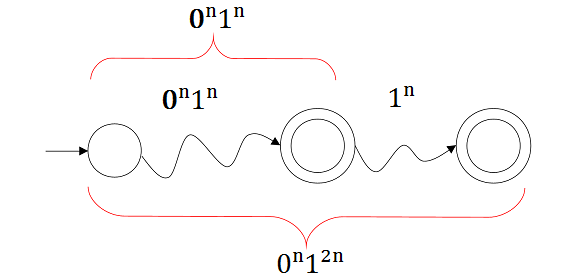
\includegraphics[width=0.5\linewidth]{image0.png}
    \caption{Автомат $M$}
    \label{fig:placeholder1}
\end{figure}

 \begin{figure}
     \centering
     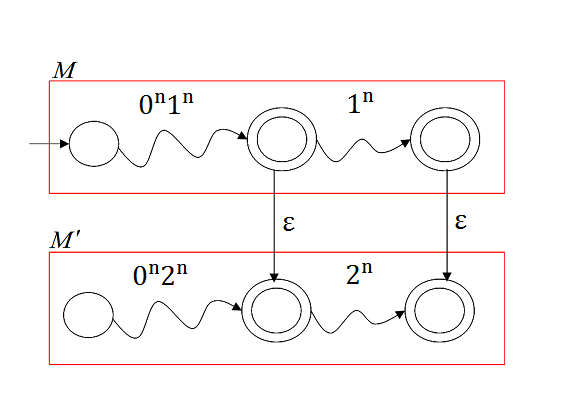
\includegraphics[width=0.5\linewidth]{image.png}
     \caption{Автомат $M''$}
     \label{fig:placeholder2}
 \end{figure}
\end{proof}

\end{document}